\section{Wednesday for MAT4002}\index{Monday_lecture}
\paragraph{Reviewing}
\begin{itemize}
\item
Edge loop based at $b\in V$:
\[
\alpha = (b,v_1,\cdots ,v_n,b)
\]
\item
Equivalence class of edge loops:
\[
[\alpha] = \{
\alpha'\mid\alpha' \sim\alpha,\text{$\alpha'$ is the edge loop based at $b$}
\}
\]
Note that $\alpha'\sim\alpha$ if they differ from finitely many elementary contractions or expansions.

For instance, let $K$ in the figure below denote a triangle:
\begin{figure}[H]
\centering
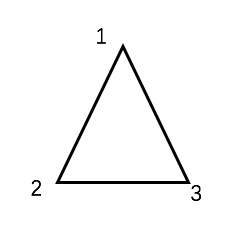
\includegraphics[width=0.2\textwidth]{week12/f_12_7}
\caption{Triangle $K$}
\label{fig:12:1}
\end{figure}
Then the canonical form of any equivalence form $[\alpha]$ can be expressed as:
\[
[\alpha] = [bcabc\cdots ab],
\]
where $a,b,c\in\{1,2,3\}$ are distinct.
\end{itemize}
\subsection{Groups $\&$ Simplicial Complices}
\begin{proposition}
The $E(K,b) = \{[\alpha]\mid\text{$\alpha$ is edge loop based at $b$}\}$ is a group, with the operation
\[
[\alpha]*[\beta] = [\alpha\cdot\beta]
\]
\end{proposition}
\begin{proof}
\begin{enumerate}
\item
Well-definedness of $*$:
\[
\alpha\sim\alpha',\beta\sim\beta'\implies
\alpha\cdot\beta\sim\alpha'\cdot\beta'
\]
\item
Associativity is clear.
\item
The identity is $e:=[b]$: for any edge loop $[\alpha]=[bv_1\cdots b]$,
\begin{align*}
[\alpha]*e&=[bv_1\cdots v_nb]*[b]\\
&=[bv_1\cdots v_nbb]\\
&=[bv_1\cdots v_nb] = [\alpha].
\end{align*}
Also, $e*[\alpha] = [\alpha]$.
\item
The inverse of any edge loop $[bv_1\cdots v_nb]$ is $[bv_n\cdots v_1b]$:
\begin{align*}
[bv_1\cdots v_nb]^{-1}*[bv_1\cdots v_nb]
&=[bv_n\cdots v_1bbv_1\cdots v_nb]\\
&=[bv_n\cdots v_1bv_1\cdots v_nb]\\
&=[bv_n\cdots v_2v_1v_2\cdots v_nb]\\
&=\cdots\\
&=[b]
\end{align*}
Similarly, $[bv_1\cdots v_nb]*[bv_1\cdots v_nb]^{-1}=[b]$.
\end{enumerate}
\end{proof}

We will see that for $K$ defined in Fig.(\ref{fig:12:1}), $E(K,1)\cong\mathbb{Z}$, in the next class.

\begin{theorem}
$E(K,b)\cong\pi_1(|K|,b)$.
\end{theorem}

This is the most difficult theorem that we have faced so far. Let's recall the simplicial approximation proposition first:
\clearpage
\begin{remark}
\begin{proposition}[Simplicial Approximation Proposition]
Suppose that $f:|K|\to|L|$ be such that for all $v\in V(K)$, there exists $g(v)\in V(L)$ satisfying 
\[
f(\text{st}_K(v))\subseteq\text{st}_L(g(v)).
\]
As a result,
\begin{enumerate}
\item
the mapping
\[
\begin{array}{ll}
g:&K\to L\\
\text{with}&v\mapsto g(v)
\end{array}
\]
is a simplicial map, i.e., for all $\sigma_K\in\Sigma_K, g(\sigma_K)\in\Sigma_L$
\item
Moreover, $|g|\simeq f.$
\end{enumerate}
Furthermore, if $A\subseteq K$ is a simplicial subcomplex such that $f(|A|)\subseteq |B|$, where $B\subseteq L$ is a simplicial subcomplex, then we can choose $g$ such that $g\mid_A:A\to B$ and the homotopy $|g|\simeq f$ sends $|A|$ to $|B|$.
\end{proposition}
\end{remark}
\begin{example}
Consider the simplicial complex $K$ and $L$ shown in the figure below:
\begin{figure}[H]
\centering
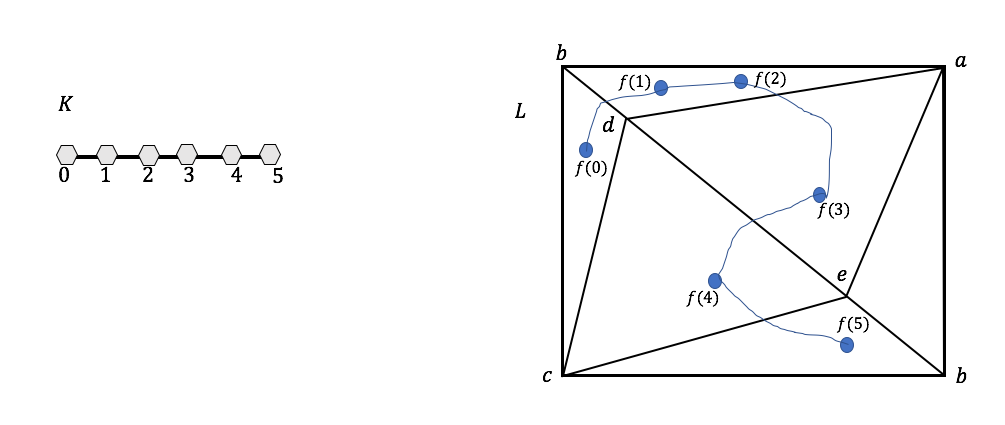
\includegraphics[width=0.8\textwidth]{week12/f_19}
\end{figure}
Let $A_1$ denote the subcomplex with $V(A_1)=\{0\},\Sigma_{A_1}=\{\{0\}\}$, and $A_2$ denote the subcomplex wit $V(A_2) = \{1,2\}$ and $\Sigma_{A_2}=\{\{1,2\},\{1\},\{2\}\}$.
Therefore, 
\[
\begin{array}{ll}
f(|A_1|)\subseteq|\Delta_{\{b,c,d\}}|,
&
f(|A_2|)\subseteq|\Delta_{\{a,b,d\}}|,
\end{array}
\]
There exists simplicial mapping $g$ with
\[
\begin{array}{llllll}
g(0)=b,
&
g(1)=b,
&
g(2)=d,
&
g(3)=e,
&
g(4)=c,
&
g(5)=c
\end{array}
\]
\end{example}

\begin{proof}
\begin{enumerate}
\item
For each edge loop $\alpha=(v_0,\dots,v_n)$ based at $b$, consider the simplicial complex 
\begin{figure}[H]
\centering
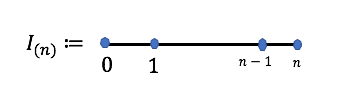
\includegraphics[width=0.5\textwidth]{week12/f_18}
\end{figure}
Together with the simplicial map
\[
\begin{array}{ll}
g_{\alpha}:&I_{(n)}\to K\\
\text{with}&g_{\alpha}(i)=v_i
\end{array}
\]
Note that it is well-defined since $\{i,i+1\}\in\Sigma_{I_{(n)}}$, and $\{v_i,v_{i+1}\}\in\Sigma_K$.

Now construct the mapping 
\[
\begin{array}{ll}
\theta:&\{\text{edge loop based at $b$}\}\to\pi_1(K,b)\\
\text{with}&\alpha\mapsto [|g_{\alpha}|]\\
\text{where}&|g_{\alpha}|:|I_{(n)}|(\cong[0,1])\to|K|\\
&|g_{\alpha}|(i/n) = v_i
\end{array}
\]
For example,
\[
\alpha = (bdeabcb), \implies
|g_\alpha|(0)=b,
|g_\alpha|(1/6) = d,
|g_\alpha|(2/6) = e,
\cdots,
|g_\alpha|(1) = b,
\]
i.e., $|g_\alpha|$ is a loop based at $b$.

Therefore, $[|g_\alpha|]\in\pi_1(|K|,b)$.
\item
Now, suppose $\alpha\sim \alpha'$ be two edge loops differ by an elemenary contraction, e.g.,
\[
\alpha'=(bdebcb)\sim\alpha=(bdeabcb).
\]
As a result, $|g_{\alpha'}|\simeq|g_{\alpha}|$ relative to $\{0,1\}$, i.e., $[|g_\alpha|]=[|g_{\alpha'}|]$.

Therefore, we have a well-defined map:
\[
\begin{array}{ll}
\tilde{\theta}:&\{\text{edge loops based at $b$}\}/\sim\to\pi_1(|K|,b)\\
\text{with}&[\alpha]\mapsto[|g_{\alpha}|]
\end{array}
\]
Therefore, $\tilde{\theta}:E(K,b)\to\pi_1(|K|,b)$ is the desired map.
\item
$\tilde{\theta}$ is a homomorphism:
it suffices to show that 
\begin{align*}
\tilde{\theta}([\alpha]*[\beta])&=\tilde{\theta}([\alpha])\tilde{\theta}([\beta]),
\end{align*}
which suffices to show $[|g_{\alpha\cdot\beta}|] = [|g_\alpha||g_{\beta}|]$, i.e., $|g_{\alpha\cdot\beta}|\simeq |g_\alpha||g_{\beta}|$.
Note that $|g_{\alpha\cdot\beta}|$ and $|g_\alpha||g_{\beta}|$ are the same path with different ``speed'', i.e., homotopy.
\item
The mapping $\tilde{\theta}$ is surjective:
Let $\ell:[0,1]\to|K|$ be a loop based at $b$.
It suffices to find an edge loop $\alpha$ such that $[|g_\alpha|]=[\ell]$, i.e., $|g_\alpha|\simeq\ell$.
\begin{enumerate}
\item
Applying the simplicial approximation theorem, there exist large $n$ and $g:I_{(n)}\to K$ such that $|g|\simeq\ell$.
Here we can choose $g:I_{(n)}\to K$ to be such that $g(\{0\})=\{b\}$, $g(\{n\})=\{b\}$, and $|g|\simeq\ell$ relative to $\{0,1\}$.
\item
Take $\alpha = (g(0),g(1),\dots,g(n))$ so that $g(0)=b=g(n)$, with $g_\alpha = g$.
Therefore, $[|g_\alpha|]=[\ell]$, and hence $\tilde{\theta}$ is surjective.
\end{enumerate}
\end{enumerate}
\end{proof}









